
%--------------------
 
\chapter{Modelo lineal Bayesiano}

En términos de modelamiento estadístico, la relación entre una variable de interés $Y$ y una matriz de variables auxiliares $\mathbf{X}$, es una de las herramientas estadísticas más utilizadas por los investigadores en los últimos tiempos. Herramientas como la regresión simple, la regresión múltiple y el análisis de varianza forman parte del arsenal de opciones que la ciencia estadística ofrece a los usuarios que van un paso más allá estableciendo relaciones de causalidad en el contexto de propio de la investigación.

Por supuesto, el enfoque bayesiano también ofrece al investigador herramientas poderosas en términos del modelamiento de relaciones causales. Siguiendo el mismo espíritu que en los anteriores capítulos, la inferencia bayesiana proporciona distribuciones posterior para los parámetros de interés y distribuciones predictivas para nuevas observaciones en cada uno de los contextos mencionados anteriormente. Como lo menciona \citeasnoun{Migon}, es muy útil adoptar la notación matricial para el desarrollo posterior del análisis bayesiano; entonces, se definen
\begin{equation*}
\mathbf{Y}=
\begin{pmatrix}
  Y_1 \\
  \vdots \\
  Y_n \\
\end{pmatrix} \ \ \ \ \ \ \ \ \ \ \text{y} \ \ \ \ \ \ \ \ \
\textbf{X}=
\begin{pmatrix}
  \mathbf{x}_1' \\
  \vdots \\
  \mathbf{x}_n' \\
\end{pmatrix}
=
\begin{pmatrix}
  x_{11} & \ldots & x_{1q} \\
  \vdots & \ddots & \vdots \\
  x_{n1} & \ldots & x_{nq} \\
\end{pmatrix}
\end{equation*}

y se supone que existe una relación de causalidad de parte de $\mathbf{X}$ reflejada en $\mathbf{Y}$ que puede ser descrita mediante el siguiente modelo probabilístico
\begin{equation}
\mathbf{Y}=\mathbf{X}\bbeta+\beps
\end{equation}

en donde $\beps=(\varepsilon_1,\ldots,\varepsilon_n)'$ es un vector aleatorio tal que cada una de sus componentes sigue una distribución de probabilidad, que en la mayoría de los casos suele ser normal. Antes de comenzar con la estipulación propia del análisis bayesiano, es necesario aclarar el papel que juegan las variables auxiliares en la inferencia estadística.

En primer lugar, nótese que el interés particular recae en la distribución del vector de $n$ variables aleatorias $\mathbf{Y}=(Y_1\ldots,Y_n)'$
condicional a la matriz de variables auxiliares $\mathbf{X}$ e indexada por el vector de parámetros de interés $\bbeta=(\beta_1,\ldots,\beta_q)'$ dada por $p(\mathbf{Y} \mid \bbeta,\mathbf{X})$.

Basado en lo anterior, es posible y suponiendo que las variables de interés son intercambiables, entonces es posible plantear el siguiente modelo poblacional
\begin{align*}
E(Y_i \mid \bbeta,\mathbf{X})&=\bbeta\mathbf{x}_{i}'=\beta_1x_{i1}+\cdots+\beta_qx_{iq}\\
Var(Y_i \mid \bbeta,\mathbf{X})&=\sigma^2
\end{align*}

para $i=1,\ldots,n$. Generalmente $\bbeta$ y $\sigma^2$ son los parámetros de interés. \citeasnoun{Gelman03} afirma que en la realidad, las observaciones incluyen realizaciones tanto de las variables de interés $Y_i$ como de las variables auxiliares $\mathbf{X}$ y por la anterior razón, el modelamiento bayesiano propiamente dicho debería incluir

\begin{enumerate}[a]
  \item Una distribución  para las variables auxiliares $\mathbf{X}$ indexada por un vector de hiperparámetros $\bphi$, dada por $p(\mathbf{X} \mid \bphi)$.
  \item Una verosimilitud conjunta de los datos observados dada por $p(\mathbf{X},\mathbf{Y} \mid \bphi,\btheta)$, en donde $\btheta=(\bbeta',\sigma^2)$ es el vector de parámetros de interés.
  \item  Por último, una distribución previa conjunta para los parámetros desconocidos dada por $p(\bphi,\btheta)$.
\end{enumerate}

Sin embargo, en un contexto estándar, los anteriores requerimientos se simplifican al suponer que los parámetros $\btheta$ y $\bphi$ son independientes previa - es decir $p(\btheta,\bphi)=p(\btheta)p(\bphi)$ - y que la distribución de las variables auxiliares es no informativa al igual que la distribución previa del parámetro $\bphi$ - es decir que $p(\bphi \mid \mathbf{X})\propto k$ . De esta manera se tiene que
\begin{align*}
p(\btheta,\bphi \mid \mathbf{Y},\mathbf{X} )&=p(\bphi \mid \mathbf{X})p(\btheta \mid \mathbf{Y},\mathbf{X})\\
&\propto p(\btheta \mid \mathbf{Y},\mathbf{X})\\
&\propto p(\btheta)p(\mathbf{Y} \mid \btheta,\mathbf{X})
\end{align*}

Por ende, de aquí en adelante vamos a referirnos a la distribución posterior de $\bbeta$ comprendiendo que la especificación de esta distribución cubre todo el ámbito probabilístico de las observaciones de las variables auxiliares.

El modelo básico y clásico asume que la verosimilitud para las variables de interés es
\begin{equation*}
\mathbf{Y} \mid \btheta,\sigma^2,\mathbf{X}\sim Normal_n(\mathbf{X}\bbeta,\sigma^2\mathbf{I}_n)
\end{equation*}

en donde $\mathbf{I}_n$ denota la matriz identidad de orden $n\times n$. Por supuesto, el modelo normal no es el único que se puede postular como verosimilitud para los datos. Existen muchos más distribuciones que serán contempladas más adelante.

\section{Modelo lineal con varianza conocida}

En términos generales, la verosimilitud del vector de variables de interés está dada por la siguiente expresión
\begin{equation}
p(\mathbf{Y} \mid \bbeta,\bSigma,\mathbf{X})\propto \exp\left\{-\frac{1}{2}(\mathbf{y}-\mathbf{X}\bbeta)'\bSigma^{-1}(\mathbf{y}-\mathbf{X}\bbeta)\right\}
\end{equation}

en donde $\bSigma$ representa la matriz de varianzas de $\mathbf{Y}$, simétrica y definida positiva. Se tiene que cada una de las entradas de la matriz de varianzas  es conocida. Suponga que la distribución previa del vector de parámetros de interés es informativa y además está regida por la siguiente estructura probabilística
\begin{equation*}
\bbeta\sim Normal_q(\mathbf{b},\mathbf{B})
\end{equation*}

Nótese que es natural asignarle a $\bbeta$ una distribución normal multivariante pues cada uno de sus componentes describe una relación numérica de la variable de interés con la correspondiente variable de información auxiliar, y por consiguiente puede tomar valores positivos o negativos, entreros o fraccionarios. Bajo este contexto se tiene el siguiente resultado.

\begin{Res}
La distribución posterior para el vector de parámetros de interés es
\begin{equation*}
\bbeta \mid \mathbf{Y},\mathbf{X},\bSigma \sim Normal_q(\mathbf{b}_q,\mathbf{B}_q)
\end{equation*}
donde
\begin{align*}
\mathbf{B}_q &= \left(\mathbf{B}^{-1}+\mathbf{X}'\bSigma^{-1}\mathbf{X}\right)^{-1}\\
\mathbf{b}_q &=\mathbf{B}_q\left(\mathbf{B}^{-1}\mathbf{b}+\mathbf{X}'\bSigma^{-1}\mathbf{Y}\right)
\end{align*}
\end{Res}

\begin{proof}
De la definición de distribución posterior, y completando cuadrados como en la demostración del Resultado 3.2.1.,  se tiene que
\begin{align*}
p(\bbeta \mid \mathbf{Y},\bSigma)&\propto
\exp\left\{-\frac{1}{2}\left[(\mathbf{y}-\mathbf{X}\bbeta)'\bSigma^{-1}(\mathbf{y}-\mathbf{X}\bbeta)
+(\bbeta-\mathbf{b})'\mathbf{B}^{-1}(\bbeta-\mathbf{b})\right]\right\}\\
&\propto
\exp\left\{-\frac{1}{2}\left[\bbeta'(\mathbf{X}'\bSigma^{-1}\mathbf{X}+\mathbf{B}^{-1})\bbeta
- 2\bbeta'(\mathbf{X}'\bSigma^{-1}\mathbf{Y}+\mathbf{B}^{-1}\mathbf{b})\right]\right\}\\
&=\exp\left\{-\frac{1}{2}\bbeta'\mathbf{B}^{-1}_q\bbeta
+ \bbeta'\mathbf{B}^{-1}_q\mathbf{b}_q\right\}\\
&\propto\exp\left\{-\frac{1}{2}\bbeta'\mathbf{B}^{-1}_q\bbeta
+ \bbeta'\mathbf{B}^{-1}_q\mathbf{b}_q
-\frac{1}{2}\mathbf{b}_q'\mathbf{B}^{-1}_q\mathbf{b}_q\right\}\\
&=\exp\left\{-\frac{1}{2}(\bbeta-\mathbf{b}_q)'\mathbf{B}^{-1}_q(\bbeta-\mathbf{b}_q)\right\}
\end{align*}
Por lo tanto, factorizando convenientemente, se encuentra una expresión idéntica a la
función de distribución de una vector aleatorio con distribución $Normal_q(\mathbf{b}_q,\mathbf{B}_q)$.
\end{proof}

Contextualizado en el modelo lineal clásico, en donde la varianza de las observaciones es constante e igual a $\sigma^2$ y se supone que no existe correlación entre ellas, entonces $\bSigma=\sigma^2\mathbf{I}_n$, y la función de verosimilitud del vector de variables de interés está dada por la siguiente expresión
\begin{equation}
p(\mathbf{Y} \mid \bbeta,\sigma^2,\mathbf{X})\propto \exp\left\{-\frac{1}{2\sigma^2}(\mathbf{y}-\mathbf{X}\bbeta)'(\mathbf{y}-\mathbf{X}\bbeta)\right\}
\end{equation}

en donde el parámetro $\sigma^2$ es conocido. La distribución posterior para el vector de parámetros de interés $\bbeta$ sería
\begin{equation*}
\bbeta \mid \mathbf{Y},\mathbf{X},\sigma^2 \sim Normal_q(\mathbf{b}_q,\mathbf{B}_q)
\end{equation*}
donde
\begin{align*}
\mathbf{B}_q &= \left(\mathbf{B}^{-1}+\frac{1}{\sigma^2}\mathbf{X}'\mathbf{X}\right)^{-1}\\
\mathbf{b}_q &=\mathbf{B}_q\left(\mathbf{B}^{-1}\mathbf{b}+\frac{1}{\sigma^2}\mathbf{X}'\mathbf{Y}\right)
\end{align*}

Nótese que si las entradas diagonales de la matriz de covarianzas $\mathbf{B}$ en la distribución previa para $\bbeta$ es muy grande, entonces $\mathbf{B}^{-1}\longrightarrow \mathbf{0}_{q\times q}$ y por lo tanto, se tiene que
\begin{align*}
\mathbf{B}_q &\longrightarrow \sigma^2(\mathbf{X}'\mathbf{X})^{-1}\\
\mathbf{b}_q &\longrightarrow (\mathbf{X}'\mathbf{X})^{-1}\mathbf{X}'\mathbf{Y}
\end{align*}

y las anteriores expresiones que coinciden con los estimadores del modelo lineal clásico usando técnicas frecuentistas como la estimación mediante la técnica de los mínimos cuadrados o por el método de máxima verosimilitud. Por lo anterior, usar valores grandes en la diagonal de la matriz $\mathbf{B}$ es una buena alternativa para cuando no se dispone ninguna información previa.

Por otro lado, cuando tenemos datos de las variables $\mathbf{Y}$ y $\mathbf{X}$ que nos sirvan como información previa, podemos ajustar una línea de regresión siguiendo la metodología de la estadística clásica, y usar las estimaciones obtenidas de los coeficientes de regresión como el parámetro $\mathbf{b}$ y usar los errores estandares de las estimaciones al cuadrado como los elementos diagonales de la matriz $\mathbf{B}$.

\begin{Eje}\label{renal_varianza_conocida}
Para ilustrar el cómo se halla la estimación bayesiana de los coeficientes de regresión, hacemos uso de los datos del puntaje del funcionamiento renal reportados en \citeasnoun{Efronims} que habían sido estudiados en el ejemplo \ref{Eje-Renal}. Estos datos pueden ser descargados de la página \url{http://statweb.stanford.edu/~ckirby/brad/LSI/datasets-and-programs/datasets.html}. En este ejemplo, vamos a estudiar el efecto de la variable edad sobre el puntaje obtenido, esto es, procedemos a ajustar la línea de regresión $y_i=\beta_0+\beta_1Edad_i+e_i$ con $i=1,\cdots,157$, usamos $\sigma^2=3.5$. Primero cargamos y examinamos los datos.
\begin{knitrout}
\definecolor{shadecolor}{rgb}{0.933, 0.933, 0.933}\color{fgcolor}\begin{kframe}
\begin{alltt}
\hlkwd{load}\hlstd{(}\hlstr{"kidneydata.Rdata"}\hlstd{)}
\hlkwd{attach}\hlstd{(}\hlstr{"kidneydata.Rdata"}\hlstd{)}
\end{alltt}


{\ttfamily\noindent\itshape\color{messagecolor}{\#\# The following object is masked \_by\_ .GlobalEnv:\\\#\# \\\#\#\ \ \ \  kidneydata}}\begin{alltt}
\hlkwd{head}\hlstd{(kidneydata)}
\end{alltt}
\begin{verbatim}
##      age   Tot
## [1,]  31  1.69
## [2,]  36 -1.41
## [3,]  24 -0.28
## [4,]  35 -0.91
## [5,]  53  3.22
## [6,]  36 -1.47
\end{verbatim}
\begin{alltt}
\hlkwd{plot}\hlstd{(kidneydata[,}\hlnum{1}\hlstd{], kidneydata[,}\hlnum{2}\hlstd{],}\hlkwc{xlab}\hlstd{=}\hlstr{"Edad"}\hlstd{,} \hlkwc{ylab}\hlstd{=}\hlstr{"Puntaje"}\hlstd{)}
\end{alltt}
\end{kframe}
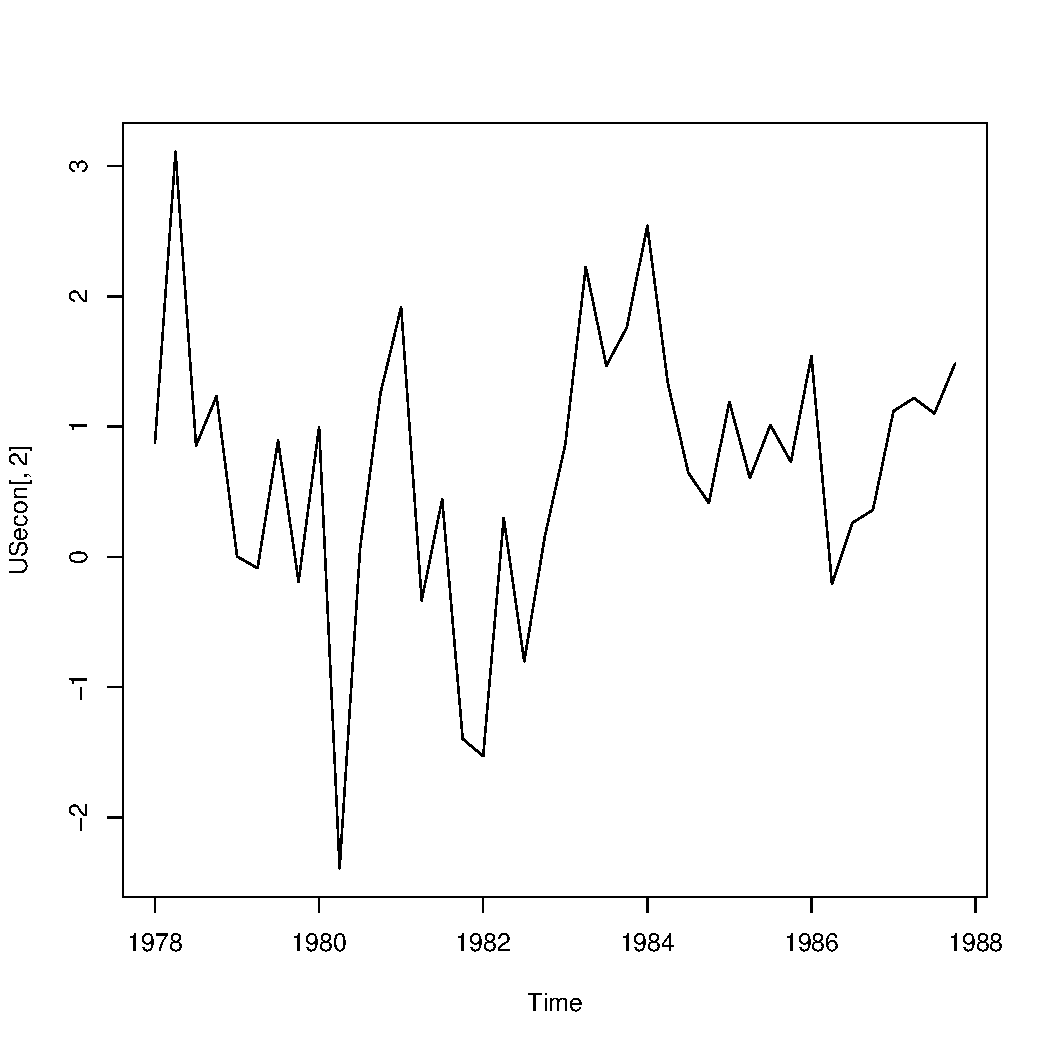
\includegraphics[width=\maxwidth]{figure/unnamed-chunk-2-1} 

\end{knitrout}
De la gráfica de dispersión se observa que a medida que la persona avance en edad, la función renal disminuye. Para realizar un análisis bayesiano sin información previa, utilizamos $\mathbf{b}=\mathbf{0}$ y $\mathbf{B}=1000\times\mathbf{I}_2$.

\colorbox{black}{\textcolor{white}{\textbf{Código JAGS}}}
\begin{knitrout}
\definecolor{shadecolor}{rgb}{0.933, 0.933, 0.933}\color{fgcolor}\begin{kframe}
\begin{alltt}
\hlstd{Regre.Model} \hlkwb{<-} \hlkwa{function}\hlstd{()\{}
  \hlkwa{for} \hlstd{(i} \hlkwa{in} \hlnum{1}\hlopt{:}\hlstd{n)}
  \hlstd{\{}
    \hlstd{y[i]} \hlopt{~} \hlkwd{dnorm}\hlstd{(mu[i],tau)}
    \hlstd{mu[i]} \hlkwb{<-} \hlstd{beta0} \hlopt{+} \hlstd{beta1}\hlopt{*}\hlstd{x[i]}
  \hlstd{\}}
  \hlcom{# Distribución previa para los parámetros}
  \hlstd{beta0} \hlopt{~} \hlkwd{dnorm}\hlstd{(}\hlnum{0}\hlstd{,} \hlnum{0.0001}\hlstd{)}
  \hlstd{beta1} \hlopt{~} \hlkwd{dnorm}\hlstd{(}\hlnum{0}\hlstd{,} \hlnum{0.0001}\hlstd{)}
  \hlstd{tau} \hlkwb{<-} \hlnum{1}\hlopt{/}\hlstd{sigma2}
\hlstd{\}}

\hlstd{y} \hlkwb{<-} \hlstd{kidneydata[,}\hlnum{2}\hlstd{]}
\hlstd{x} \hlkwb{<-} \hlstd{kidneydata[,}\hlnum{1}\hlstd{]}
\hlstd{n} \hlkwb{<-} \hlkwd{length}\hlstd{(y)}
\hlstd{sigma2} \hlkwb{<-} \hlnum{3.5}

\hlstd{Regre.Model.data} \hlkwb{<-} \hlkwd{list}\hlstd{(}\hlstr{"y"}\hlstd{,} \hlstr{"x"}\hlstd{,} \hlstr{"n"}\hlstd{,} \hlstr{"sigma2"}\hlstd{)}
\hlstd{Regre.Model.param} \hlkwb{<-} \hlkwd{c}\hlstd{(}\hlstr{"beta0"}\hlstd{,} \hlstr{"beta1"}\hlstd{)}
\hlstd{Regre.Model.inits} \hlkwb{<-} \hlkwa{function}\hlstd{()\{}
  \hlkwd{list}\hlstd{(}\hlstr{"beta0"}\hlstd{=}\hlkwd{c}\hlstd{(}\hlnum{0}\hlstd{),} \hlstr{"beta1"}\hlstd{=}\hlkwd{c}\hlstd{(}\hlnum{0}\hlstd{))}
\hlstd{\}}

\hlstd{Regre.Model.fit} \hlkwb{<-} \hlkwd{jags}\hlstd{(}\hlkwc{data}\hlstd{=Regre.Model.data,} \hlkwc{inits}\hlstd{=Regre.Model.inits,}
        \hlstd{Regre.Model.param,} \hlkwc{n.iter}\hlstd{=}\hlnum{10000}\hlstd{,} \hlkwc{n.burnin}\hlstd{=}\hlnum{1000}\hlstd{,} \hlkwc{model.file}\hlstd{=Regre.Model)}
\end{alltt}


{\ttfamily\noindent\itshape\color{messagecolor}{\#\# module glm loaded}}\begin{verbatim}
## Compiling model graph
##    Resolving undeclared variables
##    Allocating nodes
## Graph information:
##    Observed stochastic nodes: 157
##    Unobserved stochastic nodes: 2
##    Total graph size: 426
## 
## Initializing model
\end{verbatim}
\begin{alltt}
\hlkwd{print}\hlstd{(Regre.Model.fit)}
\end{alltt}
\begin{verbatim}
## Inference for Bugs model at "/var/folders/c3/jvv2xf7j2zv8xh875zp2hly40000gn/T//Rtmp6efzfU/model1b7f7b8c3e8e.txt", fit using jags,
##  3 chains, each with 10000 iterations (first 1000 discarded), n.thin = 9
##  n.sims = 3000 iterations saved
##          mu.vect sd.vect    2.5%     25%     50%     75%    98% Rhat n.eff
## beta0      2.860    0.38   2.144   2.611   2.862   3.111   3.59    1  3000
## beta1     -0.079    0.01  -0.097  -0.085  -0.079  -0.072  -0.06    1  2000
## deviance 630.920    2.04 628.933 629.480 630.295 631.710 636.22    1  3000
## 
## For each parameter, n.eff is a crude measure of effective sample size,
## and Rhat is the potential scale reduction factor (at convergence, Rhat=1).
## 
## DIC info (using the rule, pD = var(deviance)/2)
## pD = 2.1 and DIC = 633.0
## DIC is an estimate of expected predictive error (lower deviance is better).
\end{verbatim}
\end{kframe}
\end{knitrout}
El anterior procedimiento se puede llevar a cabo en \verb'R' usando los siguientes códigos. 

\colorbox{black}{\textcolor{white}{\textbf{Código R}}}
\begin{knitrout}
\definecolor{shadecolor}{rgb}{0.933, 0.933, 0.933}\color{fgcolor}\begin{kframe}
\begin{alltt}
\hlcom{# Parámetros de la distribución previa}
\hlstd{B} \hlkwb{<-} \hlkwd{diag}\hlstd{(}\hlkwd{rep}\hlstd{(}\hlnum{100}\hlstd{,}\hlnum{2}\hlstd{))}
\hlstd{b} \hlkwb{<-} \hlkwd{rep}\hlstd{(}\hlnum{0}\hlstd{,}\hlnum{2}\hlstd{)}
\hlcom{# Datos muestrales}
\hlstd{X} \hlkwb{<-} \hlkwd{cbind}\hlstd{(}\hlnum{1}\hlstd{,kidneydata[,}\hlnum{1}\hlstd{])}
\hlstd{Y} \hlkwb{<-} \hlstd{kidneydata[,}\hlnum{2}\hlstd{]}
\hlstd{sigma2} \hlkwb{<-} \hlnum{3.5}
\hlcom{# Parámetros de la distribución posterior}
\hlstd{Bq} \hlkwb{<-} \hlkwd{solve}\hlstd{(}\hlkwd{solve}\hlstd{(B)} \hlopt{+} \hlkwd{t}\hlstd{(X)}\hlopt\hlstd{X}\hlopt{/}\hlstd{sigma2)}
\hlstd{bq} \hlkwb{<-} \hlstd{Bq} \hlopt \hlstd{(}\hlkwd{solve}\hlstd{(B)}\hlopt\hlstd{b} \hlopt{+} \hlkwd{t}\hlstd{(X)}\hlopt\hlstd{Y}\hlopt{/}\hlstd{sigma2)}
\hlstd{Bq}
\end{alltt}
\begin{verbatim}
##         [,1]      [,2]
## [1,]  0.1393 -0.003216
## [2,] -0.0032  0.000088
\end{verbatim}
\begin{alltt}
\hlstd{bq}
\end{alltt}
\begin{verbatim}
##        [,1]
## [1,]  2.857
## [2,] -0.079
\end{verbatim}
\end{kframe}
\end{knitrout}
De los anteriores cálculos vemos que la distribución posterior de los parámetros $\beta_0$ y $\beta_1$ está dada por
\begin{align*}
\beta_0\mid \mathbf{Y},\mathbf{X}&\sim Normal(2.857, 0.1393)\\
\beta_1\mid \mathbf{Y},\mathbf{X}&\sim Normal(-0.079, 0.000088)\\
\end{align*}

Estas distribuciones posteriores coincide con lo encontrado por \verb'JAGS'. Para decidir si el efecto negativo de la variable edad sobre el puntaje es significativo, basta calcular un intervalo de credibildad para $\beta_1$ como:
\begin{knitrout}
\definecolor{shadecolor}{rgb}{0.933, 0.933, 0.933}\color{fgcolor}\begin{kframe}
\begin{alltt}
\hlkwd{qnorm}\hlstd{(}\hlkwd{c}\hlstd{(}\hlnum{0.025}\hlstd{,}\hlnum{0.975}\hlstd{), bq[}\hlnum{2}\hlstd{],} \hlkwd{sqrt}\hlstd{(Bq[}\hlnum{2}\hlstd{,}\hlnum{2}\hlstd{]))}
\end{alltt}
\begin{verbatim}
## [1] -0.097 -0.060
\end{verbatim}
\end{kframe}
\end{knitrout}
donde se evidencia que dicho intervalo únicamente valores negativos, por lo cual se puede concluir que el efecto de la edad sí es significativo. También podemos concluir sobre la evidencia de la hipótesis de que $\beta_1<-0.05$, esto es, con cada año de más, el punta de la función renal disminuye en más de 0.05 puntos. Para resolver esta inquietud, podemos calular $Pr(\beta_1<-0.5)$ usando la distribución posterior de $\beta_1$, así
\begin{knitrout}
\definecolor{shadecolor}{rgb}{0.933, 0.933, 0.933}\color{fgcolor}\begin{kframe}
\begin{alltt}
\hlkwd{pnorm}\hlstd{(}\hlopt{-}\hlnum{0.05}\hlstd{, bq[}\hlnum{2}\hlstd{],} \hlkwd{sqrt}\hlstd{(Bq[}\hlnum{2}\hlstd{,}\hlnum{2}\hlstd{]))}
\end{alltt}
\begin{verbatim}
## [1] 1
\end{verbatim}
\end{kframe}
\end{knitrout}
podemos concluir que la hipótesis de $\beta_1<-0.5$ es consistente con los datos. Finalmente, observamos los resultados de la estimación de la línea de regresión usando técnicas de la estadística clásica.
\begin{knitrout}
\definecolor{shadecolor}{rgb}{0.933, 0.933, 0.933}\color{fgcolor}\begin{kframe}
\begin{alltt}
\hlkwd{summary}\hlstd{(}\hlkwd{lm}\hlstd{(Y} \hlopt{~} \hlstd{X[,}\hlnum{2}\hlstd{]))}
\end{alltt}
\begin{verbatim}
## 
## Call:
## lm(formula = Y ~ X[, 2])
## 
## Residuals:
##    Min     1Q Median     3Q    Max 
## -4.202 -1.342  0.078  1.076  4.524 
## 
## Coefficients:
##             Estimate Std. Error t value           Pr(>|t|)    
## (Intercept)  2.86067    0.35956    7.96 0.0000000000003489 ***
## X[, 2]      -0.07860    0.00906   -8.68 0.0000000000000051 ***
## ---
## Signif. codes:  0 '***' 0.001 '**' 0.01 '*' 0.05 '.' 0.1 ' ' 1
## 
## Residual standard error: 1.8 on 155 degrees of freedom
## Multiple R-squared:  0.327,	Adjusted R-squared:  0.323 
## F-statistic: 75.3 on 1 and 155 DF,  p-value: 0.00000000000000514
\end{verbatim}
\end{kframe}
\end{knitrout}
Observamos que la estimación de los parámetros $\beta_0$ y $\beta_1$ es muy cercana a la estimación bayesiana, y el error estándar del enfoque clásico también es similar a la desviación estándar de la distribución posterior de los parámetros. 
\end{Eje}

En el anterior ejemplo, no se cuentan con datos que puedan servir como información previa de donde se puede obtener los parámetros de la distribución previa $\mathbf{b}$ y $\mathbf{B}$, por lo cual se tomó estos parámetros que representen esta falta de información previa. De lo contrario, se puede usar los datos que representan la información previa para ajustar una línea de regresión, tomar los coeficientes estimados para el vector $\mathbf{b}$, y en cuanto a la matriz $\mathbf{B}$, ésta se puede tomar como una matriz diagonal y usar los errores estándares del ajuste al cuadrado como elementos diagonales.

\section{Modelo lineal con varianza desconocida}

En muy raras ocasiones se conoce la estructura de dispersión de las variables de interés y ese desconocimiento de la variabilidad de las observaciones es la regla más que la excepción en una gran cantidad de situaciones de la vida real. En este contexto, es necesario modelar conjuntamente, tanto la matriz de varianzas como el vector de parámetros de interés que moldean la relación de causalidad.

\subsection{previas no informativas}

Para empezar, y siguiendo los supuestos básicos del modelo lineal general, suponga que las variables aleatorias de interés conforman una muestra aleatoria en donde no existe ninguna estructura de correlación y el parámetro de variabilidad es constante a través de todos los individuos de la muestra. de esta manera, la verosimilitud conjunta estará dada por la expresión (5.1.2) en donde, una vez más el parámetro $\sigma^2$ es desconocido.

En el caso más sencillo, se supone que la distribución previa conjunta de los parámetros de interés puede ser factorizada de la siguiente manera.
\begin{equation*}
p(\bbeta,\sigma^2)=p(\bbeta \mid \sigma^2)p(\sigma^2)
\end{equation*}

y asignando a cada uno de los parámetros de interés distribuciones previa no informativas, entonces, al igual que en capítulos anteriores, se concluye que la distribución previa no informativa para $\bbeta \mid \sigma^2$ puede ser uniforme y constante tal que $p(\bbeta \mid \sigma^2)\propto k$ y la de $\sigma^2$ tal que $p(\sigma^2)\propto 1/\sigma^2$. Basado en lo anterior, es factible asignar la siguiente distribución previa conjunta
\begin{equation*}
p(\bbeta,\sigma^2 \mid \mathbf{X})\propto\frac{1}{\sigma^2}
\end{equation*}

En este orden de ideas, es fácil comprobara que la distribución posterior conjunta de los parámetros de interés está dada por
\begin{align}
p(\bbeta,\sigma^2 \mid \mathbf{Y},\mathbf{X})&\propto
p(\mathbf{Y} \mid \bbeta,\sigma^2,\mathbf{X})p(\bbeta,\sigma^2 \mid \mathbf{X}) \notag \\
&\propto\left(\sigma^2\right)^{-n/2-1}
\exp\left\{-\frac{1}{2\sigma^2}(\mathbf{y}-\mathbf{X}\bbeta)'(\mathbf{y}-\mathbf{X}\bbeta)\right\}
\end{align}

Basados en la anterior distribución conjunta, se tienen los siguientes dos resultados que dan cuenta de las distribuciones marginales posterior para los parámetros de interés.

\begin{Res}
La distribución posterior del vector de parámetros $\bbeta$ condicionado a $\sigma^2, \mathbf{Y}, \mathbf{X}$ es
\begin{equation*}
\bbeta \mid \sigma^2, \mathbf{Y}, \mathbf{X}\sim Normal_q(\hat{\bbeta}, \sigma^2(\mathbf{X}'\mathbf{X})^{-1})
\end{equation*}

en donde $\hat{\bbeta}$ denota el vector de estimadores frecuentistas clásicos obtenidos con el método de mínimos cuadrados, dado por
\begin{equation}
\hat{\bbeta}=(\mathbf{X}'\mathbf{X})^{-1}\mathbf{X}'\mathbf{Y}
\end{equation}
\end{Res}

\begin{proof}
Utilizando la técnica del condicionamiento posterior, se tiene que de la expresión
\begin{align*}
p(\bbeta \mid \sigma^2,\mathbf{Y},\mathbf{X})&\propto p(\bbeta,\underbrace{\sigma^2}_{fijo} \mid \mathbf{Y},\mathbf{X})\\
&\propto \exp\left\{-\frac{1}{2\sigma^2}(\mathbf{y}-\mathbf{X}\bbeta)'(\mathbf{y}-\mathbf{X}\bbeta)\right\}\\
&= \exp\left\{-\frac{1}{2\sigma^2}(\mathbf{y}'\mathbf{y}-\mathbf{y}'\mathbf{X}\bbeta
-\bbeta'\mathbf{X}'\mathbf{y}+\bbeta'\mathbf{X}'\mathbf{X}\bbeta)\right\}\\
&\propto \exp\left\{-\frac{1}{2\sigma^2}(\mathbf{y}'\mathbf{X}'\mathbf{X}\mathbf{y}-\mathbf{y}'\mathbf{X}\bbeta
-\bbeta'\mathbf{X}'\mathbf{y}+\bbeta'\mathbf{X}'\mathbf{X}\bbeta)\right\}\\
&\propto \exp\left\{-\frac{1}{2\sigma^2}(\bbeta-(\mathbf{X}'\mathbf{X})^{-1}\mathbf{X}'\mathbf{y})'
(\mathbf{X}'\mathbf{X})(\bbeta-(\mathbf{X}'\mathbf{X})^{-1}\mathbf{X}'\mathbf{y})\right\}
\end{align*}
Por lo tanto, factorizando convenientemente, se encuentra una expresión idéntica a la
función de distribución de una vector aleatorio con distribución $Normal_q(\hat{\bbeta}, \sigma^2(\mathbf{X}'\mathbf{X})^{-1})$.
\end{proof}

\begin{Res}
La distribución posterior del parámetro $\sigma^2$ es
\begin{equation*}
\sigma^2 \mid  \mathbf{Y}, \mathbf{X}
\sim Inversa-Gamma \left(\frac{n-q}{2},\frac{S^2_e}{2}\right)
\end{equation*}

en donde $S^2_e=(\mathbf{Y}-\mathbf{X}\hat{\bbeta})'(\mathbf{Y}-\mathbf{X}\hat{\bbeta})$ denota la suma de cuadrados de los errores del modelo ajustado.
\end{Res}

\begin{proof}
Para encontrar la distribución posterior de $\sigma^2$ se utiliza la siguiente expresión, en virtud del conocimiento de la verosimilitud y la distribución posterior condicional de $\bbeta$,
\begin{align*}
P(\sigma^2 \mid  \mathbf{Y}, \mathbf{X})&=\frac{p(\bbeta,\sigma^2 \mid \mathbf{Y},\mathbf{X})}
{p(\bbeta \mid \sigma^2,\mathbf{Y},\mathbf{X})}\\
&\propto\left(\sigma^2\right)^{q/2-n/2-1}
\exp\left\{-\frac{1}{2\sigma^2}[(\mathbf{y}-\mathbf{X}\bbeta)'(\mathbf{y}-\mathbf{X}\bbeta)
-(\bbeta-\hat{\bbeta})'(\mathbf{X}'\mathbf{X})(\bbeta-\hat{\bbeta})]\right\}\\
&\propto\left(\sigma^2\right)^{-(n-q)/2-1}
\exp\left\{-\frac{1}{2\sigma^2}S^2_e\right\}
\end{align*}

Lo anterior se tiene, puesto que, teniendo en cuenta que
\begin{equation}
\mathbf{y}'\mathbf{X}\hat{\bbeta}=\hat{\bbeta}'\mathbf{X}'\mathbf{X}\hat{\bbeta}
\end{equation}

después de un simple desarrollo algebraico, se encuentra que
\begin{equation*}
(\mathbf{y}-\mathbf{X}\bbeta)'(\mathbf{y}-\mathbf{X}\bbeta)
-(\bbeta-\hat{\bbeta})'(\mathbf{X}'\mathbf{X})(\bbeta-\hat{\bbeta})
=\mathbf{Y}'\mathbf{Y}-\mathbf{Y}'\mathbf{X}\hat{\bbeta}
\end{equation*}

que coincide con
\begin{equation*}
S^2_e=(\mathbf{y}-\mathbf{X}\hat{\bbeta})'(\mathbf{y}-\mathbf{X}\hat{\bbeta})
=\mathbf{Y}'\mathbf{Y}-\mathbf{Y}'\mathbf{X}\hat{\bbeta}
\end{equation*}
Por lo tanto, factorizando convenientemente, se encuentra una expresión idéntica a la
función de distribución de una variable aleatoria con distribución $Gamma-inversa \left(\frac{n-q}{2},\frac{S^2_e}{2}\right)$.
\end{proof}

Al igual que en los capítulos anteriores, la simulación para este tipo de especificaciones debe tener en cuenta en primer lugar la simulación de la distribución $p(\sigma^2 \mid \mathbf{Y},\mathbf{X})$ y encontrar un valor estimado para este parámetro. Luego, se debe utilizar este valor para simular la distribución $p(\bbeta \mid \sigma^2,\mathbf{Y},\mathbf{X})$ e igualmente, encontrar un valor estimado para este parámetro.

\begin{Eje}
Retomamos los datos del puntaje de función renal que fue utlizado en el ejemplo \ref{renal_varianza_conocida} y procedemos a estimar la línea de regresión explicando el comportamiento del puntaje en función de la variable edad, asumimos que el valor de $\sigma^2$ es desconocido. Los códigos en \verb'JAGS' son como siguen:

\colorbox{black}{\textcolor{white}{\textbf{Código JAGS}}}
\begin{knitrout}
\definecolor{shadecolor}{rgb}{0.933, 0.933, 0.933}\color{fgcolor}\begin{kframe}
\begin{alltt}
\hlstd{Regre2.Model} \hlkwb{<-} \hlkwa{function}\hlstd{()\{}
  \hlkwa{for} \hlstd{(i} \hlkwa{in} \hlnum{1}\hlopt{:}\hlstd{n)}
  \hlstd{\{}
    \hlstd{y[i]} \hlopt{~} \hlkwd{dnorm}\hlstd{(mu[i], tau)}
    \hlstd{mu[i]} \hlkwb{<-} \hlstd{beta0} \hlopt{+} \hlstd{beta1}\hlopt{*}\hlstd{x[i]}
  \hlstd{\}}
  \hlcom{# Distribución previa para los parámetros}
  \hlstd{beta0} \hlopt{~} \hlkwd{dnorm}\hlstd{(}\hlnum{0}\hlstd{,} \hlnum{0.0001}\hlstd{)}
  \hlstd{beta1} \hlopt{~} \hlkwd{dnorm}\hlstd{(}\hlnum{0}\hlstd{,} \hlnum{0.0001}\hlstd{)}
  \hlstd{tau} \hlopt{~} \hlkwd{dgamma}\hlstd{(}\hlnum{0.001}\hlstd{,} \hlnum{0.001}\hlstd{)}
  \hlstd{sigma} \hlkwb{<-} \hlnum{1}\hlopt{/}\hlkwd{sqrt}\hlstd{(tau)}
\hlstd{\}}

\hlstd{y} \hlkwb{<-} \hlstd{kidneydata[,}\hlnum{2}\hlstd{]}
\hlstd{x} \hlkwb{<-} \hlstd{kidneydata[,}\hlnum{1}\hlstd{]}
\hlstd{n} \hlkwb{<-} \hlkwd{length}\hlstd{(y)}

\hlstd{Regre2.Model.data} \hlkwb{<-} \hlkwd{list}\hlstd{(}\hlstr{"y"}\hlstd{,} \hlstr{"x"}\hlstd{,} \hlstr{"n"}\hlstd{)}
\hlstd{Regre2.Model.param} \hlkwb{<-} \hlkwd{c}\hlstd{(}\hlstr{"beta0"}\hlstd{,} \hlstr{"beta1"}\hlstd{,} \hlstr{"sigma"}\hlstd{)}
\hlstd{Regre2.Model.inits} \hlkwb{<-} \hlkwa{function}\hlstd{()\{}
  \hlkwd{list}\hlstd{(}\hlstr{"beta0"}\hlstd{=}\hlkwd{c}\hlstd{(}\hlnum{0}\hlstd{),} \hlstr{"beta1"}\hlstd{=}\hlkwd{c}\hlstd{(}\hlnum{0}\hlstd{),} \hlstr{"tau"}\hlstd{=}\hlkwd{c}\hlstd{(}\hlnum{1}\hlstd{))}
\hlstd{\}}

\hlstd{Regre2.Model.fit} \hlkwb{<-} \hlkwd{jags}\hlstd{(}\hlkwc{data}\hlstd{=Regre2.Model.data,} \hlkwc{inits}\hlstd{=Regre2.Model.inits,}
                         \hlstd{Regre2.Model.param,} \hlkwc{n.iter}\hlstd{=}\hlnum{10000}\hlstd{,} \hlkwc{n.burnin}\hlstd{=}\hlnum{1000}\hlstd{,}
                         \hlkwc{model.file}\hlstd{=Regre2.Model)}
\end{alltt}
\begin{verbatim}
## Compiling model graph
##    Resolving undeclared variables
##    Allocating nodes
## Graph information:
##    Observed stochastic nodes: 157
##    Unobserved stochastic nodes: 3
##    Total graph size: 430
## 
## Initializing model
\end{verbatim}
\begin{alltt}
\hlkwd{print}\hlstd{(Regre2.Model.fit)}
\end{alltt}
\begin{verbatim}
## Inference for Bugs model at "/var/folders/c3/jvv2xf7j2zv8xh875zp2hly40000gn/T//Rtmp6efzfU/model1b7f345f1c00.txt", fit using jags,
##  3 chains, each with 10000 iterations (first 1000 discarded), n.thin = 9
##  n.sims = 3000 iterations saved
##          mu.vect sd.vect    2.5%     25%     50%     75%     98% Rhat
## beta0      2.870   0.356   2.178   2.622   2.872   3.109   3.569    1
## beta1     -0.079   0.009  -0.096  -0.085  -0.079  -0.073  -0.061    1
## sigma      1.810   0.104   1.616   1.738   1.804   1.875   2.029    1
## deviance 631.297   2.420 628.506 629.498 630.639 632.457 637.517    1
##          n.eff
## beta0     3000
## beta1     3000
## sigma     3000
## deviance  3000
## 
## For each parameter, n.eff is a crude measure of effective sample size,
## and Rhat is the potential scale reduction factor (at convergence, Rhat=1).
## 
## DIC info (using the rule, pD = var(deviance)/2)
## pD = 2.9 and DIC = 634.2
## DIC is an estimate of expected predictive error (lower deviance is better).
\end{verbatim}
\end{kframe}
\end{knitrout}
Los anteriores cálculos se pueden implementar en \verb'R' con los siguientes códigos:

\colorbox{black}{\textcolor{white}{\textbf{Código R}}}
\begin{knitrout}
\definecolor{shadecolor}{rgb}{0.933, 0.933, 0.933}\color{fgcolor}\begin{kframe}
\begin{alltt}
\hlkwd{library}\hlstd{(MCMCpack)}
\end{alltt}


{\ttfamily\noindent\itshape\color{messagecolor}{\#\# Loading required package: MASS}}

{\ttfamily\noindent\itshape\color{messagecolor}{\#\# \#\#\\\#\# \#\# Markov Chain Monte Carlo Package (MCMCpack)}}

{\ttfamily\noindent\itshape\color{messagecolor}{\#\# \#\# Copyright (C) 2003-2016 Andrew D. Martin, Kevin M. Quinn, and Jong Hee Park}}

{\ttfamily\noindent\itshape\color{messagecolor}{\#\# \#\#\\\#\# \#\# Support provided by the U.S. National Science Foundation}}

{\ttfamily\noindent\itshape\color{messagecolor}{\#\# \#\# (Grants SES-0350646 and SES-0350613)\\\#\# \#\#}}\begin{alltt}
\hlkwd{library}\hlstd{(mvtnorm)}
\hlcom{# Datos muestrales}
\hlstd{X} \hlkwb{<-} \hlkwd{cbind}\hlstd{(}\hlnum{1}\hlstd{,kidneydata[,}\hlnum{1}\hlstd{])}
\hlstd{Y} \hlkwb{<-} \hlstd{kidneydata[,}\hlnum{2}\hlstd{]}
\hlstd{q} \hlkwb{<-} \hlnum{2}

\hlstd{n.sim} \hlkwb{<-} \hlnum{20000}
\hlstd{beta.hat} \hlkwb{<-} \hlkwd{solve}\hlstd{(}\hlkwd{t}\hlstd{(X)}\hlopt\hlstd{X)}\hlopt\hlkwd{t}\hlstd{(X)}\hlopt\hlstd{Y}
\hlstd{S2.e} \hlkwb{<-} \hlkwd{sum}\hlstd{((Y}\hlopt{-}\hlstd{X}\hlopt\hlstd{beta.hat)}\hlopt{^}\hlnum{2}\hlstd{)}
\hlcom{# Simular valores para la varianza}
\hlstd{sigma2.res} \hlkwb{<-} \hlkwd{rinvgamma}\hlstd{(n.sim, (n}\hlopt{-}\hlstd{q)}\hlopt{/}\hlnum{2}\hlstd{, S2.e}\hlopt{/}\hlnum{2}\hlstd{)}
\hlcom{# Simular valores para los coeficientes de regresión}
\hlstd{beta.res} \hlkwb{<-} \hlkwd{matrix}\hlstd{(}\hlnum{NA}\hlstd{,n.sim,q)}
\hlkwa{for}\hlstd{(i} \hlkwa{in} \hlnum{1}\hlopt{:}\hlstd{n.sim)\{}
  \hlstd{beta.res[i,]} \hlkwb{<-} \hlkwd{rmvnorm}\hlstd{(}\hlnum{1}\hlstd{, beta.hat, sigma2.res[i]}\hlopt{*}\hlkwd{solve}\hlstd{(}\hlkwd{t}\hlstd{(X)}\hlopt\hlstd{X))}
\hlstd{\}}
\end{alltt}
\end{kframe}
\end{knitrout}
Una vez concludo el proceso de computación, procedemos a calcular las estimaciones de $\sigma^2$, $\sigma$, $\beta_0$ y $\beta_1$. Los intervalos de credibilidad pueden ser calculados como los percentiles muestrales de los valores simulados para cada parámetro.
\begin{knitrout}
\definecolor{shadecolor}{rgb}{0.933, 0.933, 0.933}\color{fgcolor}\begin{kframe}
\begin{alltt}
\hlcom{# Estimaciones puntuales}
\hlkwd{mean}\hlstd{(sigma2.res)}
\end{alltt}
\begin{verbatim}
## [1] 3.3
\end{verbatim}
\begin{alltt}
\hlkwd{mean}\hlstd{(}\hlkwd{sqrt}\hlstd{(sigma2.res))}
\end{alltt}
\begin{verbatim}
## [1] 1.8
\end{verbatim}
\begin{alltt}
\hlkwd{colMeans}\hlstd{(beta.res)}
\end{alltt}
\begin{verbatim}
## [1]  2.860 -0.079
\end{verbatim}
\begin{alltt}
\hlkwd{sd}\hlstd{(beta.res[,}\hlnum{1}\hlstd{])}
\end{alltt}
\begin{verbatim}
## [1] 0.36
\end{verbatim}
\begin{alltt}
\hlkwd{sd}\hlstd{(beta.res[,}\hlnum{2}\hlstd{])}
\end{alltt}
\begin{verbatim}
## [1] 0.0091
\end{verbatim}
\end{kframe}
\end{knitrout}
Por otro lado, obtenemos la estimación del modelo con la estadística clásica
\begin{knitrout}
\definecolor{shadecolor}{rgb}{0.933, 0.933, 0.933}\color{fgcolor}\begin{kframe}
\begin{alltt}
\hlkwd{summary}\hlstd{(}\hlkwd{lm}\hlstd{(Y} \hlopt{~} \hlstd{X[,}\hlnum{2}\hlstd{]))}
\end{alltt}
\begin{verbatim}
## 
## Call:
## lm(formula = Y ~ X[, 2])
## 
## Residuals:
##    Min     1Q Median     3Q    Max 
## -4.202 -1.342  0.078  1.076  4.524 
## 
## Coefficients:
##             Estimate Std. Error t value           Pr(>|t|)    
## (Intercept)  2.86067    0.35956    7.96 0.0000000000003489 ***
## X[, 2]      -0.07860    0.00906   -8.68 0.0000000000000051 ***
## ---
## Signif. codes:  0 '***' 0.001 '**' 0.01 '*' 0.05 '.' 0.1 ' ' 1
## 
## Residual standard error: 1.8 on 155 degrees of freedom
## Multiple R-squared:  0.327,	Adjusted R-squared:  0.323 
## F-statistic: 75.3 on 1 and 155 DF,  p-value: 0.00000000000000514
\end{verbatim}
\end{kframe}
\end{knitrout}
Observamos que la estimación de $\beta_0$, $\beta_1$ y $\sigma$ obtenido de los dos enfoques son muy similares.
\end{Eje}

\subsection{previas informativas}

Esta sección tiene dos acepciones: la primera en donde la distribución de los parámetros de interés puede ser descompuesta como el producto dependiente de dos distribuciones, y la otro, por supuesto, cuando se considera que los parámetros de interés son independientes previa. Sin embargo, para cade uno de los dos casos, es necesario reescribir la verosimilitud de las observaciones para poder obtener resultados conjugados.

En primer lugar, se definen las siguientes cantidades, las cuales se habían utilizado indirectamente en secciones anteriores pero que serán de interés para el tratamiento riguroso de las distribuciones posterior en este apartado. Luego, se define la \emph{suma de cuadrados del error de estimación de los parámetros de interés} ponderado por las variables de información auxiliar como
\begin{equation}
Q(\bbeta)=(\bbeta-\hat{\bbeta})'(\mathbf{X}'\mathbf{X})(\bbeta-\hat{\bbeta})
\end{equation}

donde $\hat{\bbeta}$ está dado por la expresión (5.2.2). Por otro lado, se define la \emph{suma de cuadrados del error de predicción} de las observaciones bajo el modelo lineal general dado por la siguiente expresión
\begin{equation}
S^2_e=(\mathbf{y}-\mathbf{X}\hat{\bbeta})'(\mathbf{y}-\mathbf{X}\hat{\bbeta})
\end{equation}

Con las anteriores expresiones es posible plantear la siguiente identidad que fue utilizada en la demostración del Resultado 5.2.3.
\begin{equation}
Q(\bbeta)+S^2_e=(\mathbf{y}-\mathbf{X}\bbeta)'(\mathbf{y}-\mathbf{X}\bbeta)
\end{equation}

Nótese que con esta expresión es posible reescribir la verosimilitud de las observaciones dada por la expresión (5.2.1) de la siguiente manera

\begin{equation}
p(\mathbf{Y} \mid \bbeta,\sigma^2,\mathbf{X})\propto (\sigma^2)^{-n/2} \exp\left\{-\frac{1}{2\sigma^2}\left(Q(\bbeta)+S^2_e\right)\right\}
\end{equation}

Antes de plantear las distirbuciones previa para los parámetros de interés, nótese que a través de este texto, cuando se trata de modelos con múltiples parámetros de interés, siempre se han planteado dos grandes posibilidades: que los parámetros sean dependientes previa y por supuesto, que los parámetros sean independientes previa. El tratamiento de ambos escenarios es diferente y vamos a estudiar cada caso con detenimiento.

\subsubsection*{Parámetros dependientes}

Los parámetros de interés son $\bbeta$ y $\sigma^2$ y su distribuciones previa conjunta se supone que está dada por
\begin{equation*}
p(\bbeta,\sigma^2)=p(\bbeta \mid \sigma^2)p(\sigma^2)
\end{equation*}

Específicamente, la distribución previa del parámetro $\bbeta$ condicionada a $\sigma^2$ es informativa y está regida por la siguiente estructura probabilística
\begin{equation*}
\bbeta \mid \sigma^2 \sim Normal_q(\mathbf{b},\sigma^2\mathbf{B})
\end{equation*}

en donde $\mathbf{b}$ es un vector de medias y $\mathbf{B}$ es una matriz de varianzas simétrica y definida positiva. Por otro lado, la distribución previa del parámetro $\sigma^2$ también se considera informativa y dada por
\begin{equation*}
\sigma^2 \sim Inversa-Gamma\left( \frac{n_0}{2}, \frac{n_0\sigma^2_0}{2} \right)
\end{equation*}

Bajo este marco de referencia se tienen los siguientes resultados.

\begin{Res}
La distribución posterior conjunta de los parámetros de interés $\bbeta,\sigma^2$ está dada por
\begin{align}
p(\bbeta,\sigma^2 \mid \mathbf{Y},\mathbf{X})
&=(\sigma^2)^{-q/2}
\exp\left\{-\frac{1}{2\sigma^2}(\bbeta-\mathbf{b}_q)'\mathbf{B}_q^{-1}(\bbeta-\mathbf{b}_q)\right\}
\notag
\\ &\hspace{3cm} \times
(\sigma^2)^{-n_1/2-1}
\exp\left\{-\frac{n_1\sigma^2_1}{2\sigma^2}\right\}
\end{align}
donde
\begin{align*}
\mathbf{B}_q &= \left(\mathbf{B}^{-1}+\mathbf{X}'\mathbf{X}\right)^{-1}\\
\mathbf{b}_q &=\mathbf{B}_q\left(\mathbf{B}^{-1}\mathbf{b}+\mathbf{X}'\mathbf{Y}\right)
\end{align*}

y además
\begin{align*}
n_1&=n_0+n\\
n_1\sigma^2_1&=
n_0\sigma^2_0+(\mathbf{Y}-\mathbf{X}\mathbf{b}_q)'\mathbf{Y}+(\mathbf{b}-\mathbf{b}_q)'\mathbf{B}^{-1}\mathbf{b}
\end{align*}
\end{Res}

\begin{proof}
Antes de empezar con la prueba formal del resultado, es necesario verificar las siguientes identidades
\begin{align}\label{5.2.9}
(\bbeta-\mathbf{b})'\mathbf{B}^{-1}(\bbeta-\mathbf{b})+Q(\bbeta)&=
(\bbeta-\mathbf{b}_q)'\mathbf{B}^{-1}_q(\bbeta-\mathbf{b}_q)+\mathbf{b}'\mathbf{B}^{-1}\mathbf{b}
\notag \\
&\hspace{2cm}
+\hat{\bbeta}'\mathbf{X}'\mathbf{X}\hat{\bbeta}
-\mathbf{b}'_q\mathbf{B}_q^{-1}\mathbf{b}_q
\end{align}

que se tiene puesto que
\begin{align*}
&(\bbeta-\mathbf{b})'\mathbf{B}^{-1}(\bbeta-\mathbf{b})+Q(\bbeta)\\
&=\bbeta'\mathbf{B}^{-1}\bbeta-2\bbeta'\mathbf{B}^{-1}\mathbf{b}+\mathbf{b}'\mathbf{B}^{-1}\mathbf{b}+\bbeta \mathbf{X}'\mathbf{X}\bbeta
-2\bbeta'\mathbf{X}'\mathbf{X} \hat{\bbeta}+\hat{\bbeta}'\mathbf{X}'\mathbf{X} \hat{\bbeta}\\
&=\bbeta'(\mathbf{B}^{-1}+\mathbf{X}'\mathbf{X})\bbeta-2\bbeta'(\mathbf{B}^{-1}\mathbf{b}+\mathbf{X}'\mathbf{X}\hat{\bbeta})+
\mathbf{b}'\mathbf{B}^{-1}\mathbf{b}+\hat{\bbeta}'\mathbf{X}'\mathbf{X} \hat{\bbeta}\\
&=\bbeta'(\mathbf{B}^{-1}_q)\bbeta-2\bbeta'(\mathbf{B}^{-1}\mathbf{b}+\mathbf{X}'\mathbf{Y})+
\mathbf{b}'\mathbf{B}^{-1}\mathbf{b}+\hat{\bbeta}'\mathbf{X}'\mathbf{X} \hat{\bbeta}\\
&=\bbeta'(\mathbf{B}^{-1}_q)\bbeta-2\bbeta'\mathbf{B}^{-1}_qb_q+
\mathbf{b}'\mathbf{B}^{-1}\mathbf{b}+\hat{\bbeta}'\mathbf{X}'\mathbf{X} \hat{\bbeta}\\
&=\bbeta'(\mathbf{B}^{-1}_q)\bbeta-2\bbeta'\mathbf{B}^{-1}_qb_q+\mathbf{b}_q'\mathbf{B}_q^{-1}\mathbf{b}_q
\mathbf{b}'\mathbf{B}^{-1}\mathbf{b}+\hat{\bbeta}'\mathbf{X}'\mathbf{X} \hat{\bbeta}-\mathbf{b}_q'\mathbf{B}_q^{-1}\mathbf{b}_q\\
&=(\bbeta-\mathbf{b}_q)'\mathbf{B}^{-1}_q(\bbeta-\mathbf{b}_q)+\mathbf{b}'\mathbf{B}^{-1}\mathbf{b}
+\hat{\bbeta}'\mathbf{X}'\mathbf{X}\hat{\bbeta}
-\mathbf{b}'_q\mathbf{B}_q^{-1}\mathbf{b}_q
\end{align*}

Por otro lado, debe notarse que
\begin{align}\label{5.2.10}
n_0\sigma_0^2+S^2_e+\mathbf{b}'\mathbf{B}^{-1}\mathbf{b}+\hat{\bbeta}'\mathbf{X}'\mathbf{X}\hat{\bbeta}
-\mathbf{b}'_q\mathbf{B}_q^{-1}\mathbf{b}_q=n_1\sigma_1^2
\end{align}

La anterior igualdad resulta de
\begin{align*}
&n_0\sigma_0^2+S^2_e+\mathbf{b}'\mathbf{B}^{-1}\mathbf{b}+\hat{\bbeta}'\mathbf{X}'\mathbf{X}\hat{\bbeta}
-\mathbf{b}'_q\mathbf{B}_q^{-1}\mathbf{b}_q\\
&=n_0\sigma_0^2+\mathbf{Y}'\mathbf{Y}-2\mathbf{Y}'\mathbf{X}\hat{\bbeta}+\hat{\bbeta}'\mathbf{X}'\mathbf{X}\hat{\bbeta}
+\mathbf{b}'\mathbf{B}^{-1}\mathbf{b}\\
&\hspace{2cm}
+\hat{\bbeta}'\mathbf{X}'\mathbf{X}\hat{\bbeta}
-\mathbf{b}'_q\mathbf{B}_q^{-1}\mathbf{B}_q(\mathbf{B}^{-1}\mathbf{b}+\mathbf{X}'\mathbf{Y})\\
&=n_0\sigma_0^2+\mathbf{Y}'\mathbf{Y}-2\hat{\bbeta}'\mathbf{X}'\mathbf{X}\hat{\bbeta}
+\hat{\bbeta}'\mathbf{X}'\mathbf{X}\hat{\bbeta}
+\mathbf{b}'\mathbf{B}^{-1}\mathbf{b}\\
&\hspace{2cm}
+\hat{\bbeta}'\mathbf{X}'\mathbf{X}\hat{\bbeta}
-\mathbf{b}'_q(\mathbf{B}^{-1}\mathbf{b}+\mathbf{X}'\mathbf{Y})\\
&=n_0\sigma_0^2+\mathbf{Y}'\mathbf{Y}-\mathbf{b}'_q\mathbf{X}'\mathbf{Y}+\mathbf{b}'\mathbf{B}^{-1}\mathbf{b}
-\mathbf{b}'_q\mathbf{B}^{-1}\mathbf{b}\\
&=n_0\sigma_0^2+(\mathbf{Y}-\mathbf{X}\mathbf{b}_q)'\mathbf{Y}+(\mathbf{b}'-\mathbf{b}_q'\mathbf{B}^{-1})\mathbf{b}\\
&=n_1\sigma_1^2
\end{align*}

Utilizando las expresiones (\ref{5.2.9}) y (\ref{5.2.10}) logra concluirse que
\begin{align}\label{5.2.11}
&Q(\bbeta)+S^2_e+(\bbeta-\mathbf{b})'\mathbf{B}^{-1}(\bbeta-\mathbf{b})+n_0\sigma^2_0\notag\\
&\hspace{3cm}
=(\bbeta-\mathbf{b}_q)'\mathbf{B}^{-1}_q(\bbeta-\mathbf{b}_q)+n_1\sigma_1^2
\end{align}

Después de haber probado las anteriores igualdades, el desarrollo de la prueba es más sencillo. Puesto que ahora, de la definición de distribución posterior, al utilizar la identidad dada por la expresión (\ref{5.2.11}), se tiene que

\begin{align*}
p(\bbeta,\sigma^2 \mid \mathbf{Y},\mathbf{X})&\propto p(\mathbf{Y} \mid \bbeta,\sigma^2,\mathbf{X})p(\bbeta,\sigma^2)\\
&\propto \left(\sigma^2\right)^{-\frac{q+n+n_0}{2}-1}\\
&\hspace{0cm}\times
\exp\left\{-\frac{1}{2\sigma^2}
\left[Q(\bbeta)+S^2_e+(\bbeta-\mathbf{b})'\mathbf{B}^{-1}(\bbeta-\mathbf{b})+n_0\sigma^2_0\right]
\right\}\\
&= \left(\sigma^2\right)^{-\frac{q+n+n_0}{2}-1}\\
&\hspace{2cm}\times
\exp\left\{-\frac{1}{2\sigma^2}
\left[(\bbeta-\mathbf{b}_q)'\mathbf{B}^{-1}_q(\bbeta-\mathbf{b}_q)+n_1\sigma_1^2 \right]
\right\}\\
&= \left(\sigma^2\right)^{-\frac{q}{2}}
\exp\left\{-\frac{1}{2\sigma^2}
\left[(\bbeta-\mathbf{b}_q)'\mathbf{B}^{-1}_q(\bbeta-\mathbf{b}_q)\right]
\right\}\\
&\hspace{2cm}\times
\left(\sigma^2\right)^{-\frac{n_1}{2}-1}
\exp\left\{-\frac{n_1}{2\sigma^2}\sigma_1^2 \right\}
\end{align*}
con lo que se concluye la prueba del resultado.
\end{proof}

La distribución posterior conjunta de los parámetros de interés tiene la forma de la distribución Normal-Gamma y es fácil demostrar que ésta es conjugada. Además, acudiendo a las técnicas bien conocidas de condicionamiento posterior e integración analítica se encuentran las distribuciones posterior de cada una de los parámetros de interés enmarcadas en los siguientes resultados.

\begin{Res}
La distribución posterior del vector de parámetros $\bbeta$ condicionada a $\sigma^2,\mathbf{Y},\mathbf{X}$ es
\begin{equation*}
\bbeta \mid \sigma^2,\mathbf{Y},\mathbf{X} \sim Normal_q(\mathbf{b}_q,\sigma^2\mathbf{B}_q)
\end{equation*}
\end{Res}

\begin{proof}
Para encontrar la distribución posterior del vector de parámetros $bbeta$, el cual depende previa del parámetro $\sigma^2$, es necesario recurrir al condicionamiento posterior notando que
\begin{equation*}
p(\bbeta \mid \sigma^2,\mathbf{Y},\mathbf{X})=p(\bbeta,\underbrace{\sigma^2}_{fijo} \mid \mathbf{Y},\mathbf{X})
\end{equation*}

Por lo tanto, de la distribución posterior conjunta dada por (5.2.8) e incorporando los términos que no depende de $\bbeta$ en la constante de proporcionalidad, se tiene fácilmente que
\begin{equation*}
p(\bbeta \mid \sigma^2,\mathbf{Y},\mathbf{X})\propto
\left(\sigma^2\right)^{-\frac{q}{2}}
\exp\left\{-\frac{1}{2\sigma^2}
\left[(\bbeta-\mathbf{b}_q)'\mathbf{B}^{-1}_q(\bbeta-\mathbf{b}_q)\right]
\right\}
\end{equation*}

De la anterior igualdad, y factorizando convenientemente, se encuentra una expresión idéntica a la función de distribución de una vector aleatorio con distribución $Normal_q(\mathbf{b}_q,\sigma^2\mathbf{B}_q)$.
\end{proof}

\begin{Res}
La distribución posterior del parámetro $\sigma^2$ condicionada es
\begin{equation*}
\sigma^2 \mid \mathbf{Y},\mathbf{X} \sim Inversa-Gamma\left(\frac{n_1}{2},\frac{\sigma^2_1}{2}\right)
\end{equation*}
\end{Res}

\begin{proof}
En este caso es posible servirse de la técnica de integración analítica de la siguiente manera
\begin{align*}
p(\sigma^2 \mid \mathbf{Y},\mathbf{X})&=\int p(\bbeta,\sigma^2 \mid \mathbf{Y},\mathbf{X})\ d\bbeta\\
&\propto\left(\sigma^2\right)^{-\frac{n_1}{2}-1}
\exp\left\{-\frac{n_1}{2\sigma^2}\sigma_1^2 \right\}\\
&\hspace{1cm}\times
\int\left(2\pi \sigma^2\right)^{-\frac{q}{2}}
\exp\left\{-\frac{1}{2\sigma^2}
\left[(\bbeta-\mathbf{b}_q)'\mathbf{B}^{-1}_q(\bbeta-\mathbf{b}_q)\right]\right\}\ d\bbeta\\
&=\left(\sigma^2\right)^{-\frac{n_1}{2}-1}
\exp\left\{-\frac{n_1}{2\sigma^2}\sigma_1^2 \right\}
\end{align*}

Por lo tanto, factorizando convenientemente, se encuentra una expresión idéntica a la función de distribución de una variable aleatoria con distribución $Inversa-Gamma\left(\frac{n_1}{2},\frac{\sigma^2_1}{2}\right)$.
\end{proof}

\subsubsection*{Parámetros dependientes}

\citeasnoun{Gamer06} menciona que existe una mayor dificultad para encontrar distribuciones conjugadas conforme el modelo se torna más complejo y la dimensión del espacio de parámetros crece. En esta ocasión se considera que los parámetros son independientes previa; es decir que la distribución previa conjunta está dada por
\begin{equation*}
p(\bbeta,\sigma^2)=p(\bbeta)p(\sigma^2)
\end{equation*}

Como es natural, la distribución previa del vector de parámetros $\bbeta$ es normal, aunque esta vez la matriz de varianzas no va a depender del otro parámetro $\sigma^2$, por lo tanto se tiene que
\begin{equation*}
\bbeta \sim Normal_q(\mathbf{b},\mathbf{B})
\end{equation*}

Igualmente, el parámetro $\sigma^2$ no depende de $\bbeta$ y es posible asignarle la siguiente distribución previa
\begin{equation*}
\sigma^2\sim Inversa-Gamma\left(\frac{n_0}{2},\frac{n_0\sigma^2_0}{2}\right)
\end{equation*}

Empleando la forma de la verosimilitud dada en la expresión (5.2.7), fácilmente se concluye que la distribución posterior conjunta puede ser escrita como
\begin{align}
p(\bbeta,\sigma^2 \mid \mathbf{Y},\mathbf{X})&\propto p(\mathbf{Y} \mid \bbeta,\sigma^2)p(\bbeta)p(\sigma^2)\notag \\
&\propto (\sigma^2)^{-n/2} \exp\left\{-\frac{1}{2\sigma^2}\left(Q(\bbeta)+S^2_e\right)\right\}\notag\\
&\times
\exp\left\{-\frac{1}{2}(\bbeta-\mathbf{b})'\mathbf{B}^{-1}(\bbeta-\mathbf{b})\right\}
(\sigma^2)^{-n_0/2-1} \exp\left\{-\frac{n_0\sigma^2_0}{2\sigma^2}\right\}\notag\\
&=(\sigma^2)^{-\frac{n+n_0}{2}-1}
\exp\left\{-\frac{1}{2\sigma^2}\left[Q(\bbeta)+S^2_e+n_0\sigma^2_0\right]\right\} \notag \\
&\times
\exp\left\{-\frac{1}{2}(\bbeta-\mathbf{b})'\mathbf{B}^{-1}(\bbeta-\mathbf{b})\right\}
\end{align}

\citeasnoun{Gamer06} concluye que no es posible reconocer la anterior distribución posterior como perteneciente a alguna forma analítica conocida y por tanto no es una distribución conjugada (aunque la distribución previa sea un caso particular de esta última distribución).

Una vez más, dado esto, no es posible utilizar la técnica de integración analítica para encontrar las distribuciones posterior marginales de los parámetros de interés. Sin embargo, a pesar de las anteriores razones, sí es posible encontrar fácilmente tales distribuciones marginales utilizando el condicionamiento posterior.

\begin{Res}
La distribución posterior del parámetro $\bbeta$ condicionado a $\sigma^2,\mathbf{Y},\mathbf{X}$ es
\begin{equation*}
\bbeta \mid \sigma^2,\mathbf{Y},\mathbf{X} \sim Normal_q(\mathbf{b}_q,\mathbf{B}_q)
\end{equation*}

donde
\begin{align*}
\mathbf{B}_q &= \left(\mathbf{B}^{-1}+\frac{1}{\sigma^2}\mathbf{X}'\mathbf{X}\right)^{-1}\\
\mathbf{b}_q &=\mathbf{B}_q\left(\mathbf{B}^{-1}\mathbf{b}+\frac{1}{\sigma^2}\mathbf{X}'\mathbf{Y}\right)
\end{align*}
\end{Res}

\begin{proof}
Utilizando el condicionamiento posterior en la expresión (5.2.12), se tiene que

\begin{align*}
p(\bbeta \mid \sigma^2,\mathbf{Y},\mathbf{X})&\propto
p(\bbeta,\underbrace{\sigma^2}_{fijo} \mid \mathbf{Y},\mathbf{X})\\
&\propto \exp\left\{-\frac{1}{2}
\left[\frac{1}{\sigma^2}Q(\bbeta)+(\bbeta-\mathbf{b})'\mathbf{B}^{-1}(\bbeta-\mathbf{b})\right]\right\}\\
&= \exp\left\{-\frac{1}{2}
\left[\frac{1}{\sigma^2}(\bbeta-\hat{\bbeta})'(\mathbf{X}'\mathbf{X})(\bbeta-\hat{\bbeta})
+(\bbeta-\mathbf{b})'\mathbf{B}^{-1}(\bbeta-\mathbf{b})\right]\right\}\\
&\propto \exp\left\{-\frac{1}{2}
\left[\frac{1}{\sigma^2}\bbeta'\mathbf{X}'\mathbf{X}\bbeta-
\frac{2}{\sigma^2}\bbeta'\mathbf{X}'\mathbf{X}\hat{\bbeta}
+\bbeta'\mathbf{B}^{-1}\bbeta-2\bbeta'\mathbf{b}\mathbf{B}^{-1}\right]\right\}\\
&=\propto \exp\left\{-\frac{1}{2}
\left[\bbeta'\left( \frac{1}{\sigma^2}\mathbf{X}'\mathbf{X}+\mathbf{B}^{-1}\right)\bbeta
-2\bbeta'\left(\frac{1}{\sigma^2}\mathbf{X}'\mathbf{Y}+\mathbf{B}^{-1}\mathbf{b}\right)\right]\right\}\\
&= \exp\left\{-\frac{1}{2}
\left[\bbeta'\mathbf{B}^{-1}_q\bbeta-2\bbeta'\mathbf{B}^{-1}_q\mathbf{b}_q\right]\right\}\\
&\propto \exp\left\{-\frac{1}{2}
\left[\bbeta'\mathbf{B}^{-1}_q\bbeta-2\bbeta'\mathbf{B}^{-1}_q\mathbf{b}_q
+\mathbf{b}_q'\mathbf{B}^{-1}_q\mathbf{b}_q\right]\right\}\\
&\propto \exp\left\{-\frac{1}{2}
(\bbeta-\mathbf{b}_q)'\mathbf{B}^{-1}_q(\bbeta-\mathbf{b}_q)\right\}
\end{align*}
Por lo tanto, factorizando convenientemente, se encuentra una expresión idéntica a la función de distribución de un vector aleatorio con distribución $Normal_q(\mathbf{b}_q,\mathbf{B}_q)$.
\end{proof}

\begin{Res}
La distribución posterior del parámetro $\sigma^2$ condicionado a $\bbeta,\mathbf{Y},\mathbf{X}$ es
\begin{equation*}
\sigma^2 \mid \bbeta,\mathbf{Y},\mathbf{X} \sim Inversa-Gamma\left( \frac{n_1}{2}, \frac{n_1\sigma_{\bbeta}^2}{2}  \right)
\end{equation*}

donde $n_1=n+n_0$
\begin{align*}
n_1\sigma_{\bbeta}^2=Q(\bbeta)+S^2_e+n_0\sigma^2_0
\end{align*}
\end{Res}

\begin{proof}
Utilizando el condicionamiento posterior sobre la expresión (5.2.12), se tiene que
\begin{align*}
p(\sigma^2 \mid \bbeta,\mathbf{Y},\mathbf{X})&\propto
p(\sigma^2,\underbrace{\bbeta}_{fijo} \mid \mathbf{Y},\mathbf{X})\\
&\propto(\sigma^2)^{-\frac{n+n_0}{2}-1}
\exp\left\{-\frac{1}{2\sigma^2}\left[Q(\bbeta)+S^2_e+n_0\sigma^2_0\right]\right\}\\
&\propto(\sigma^2)^{-\frac{n_1}{2}-1}
\exp\left\{-\frac{n_1\sigma_{\bbeta}^2}{2\sigma^2}\right\}
\end{align*}
Por lo tanto, factorizando convenientemente, se encuentra una expresión idéntica a la función de distribución de un vector aleatorio con distribución $Inversa-Gamma\left( \frac{n_1}{2}, \frac{n_1\sigma_{\bbeta}^2}{2}  \right)$.
\end{proof}

\citeasnoun{Gamer06} afirma que las anteriores especificaciones tienen una altísima relevancia práctica y es concebible fijar un conjunto de valores iniciales e ir actualizando las estimaciones acerca de los parámetros de interés.

